\chapter{Implementation}
\label{chapter:implementation}
\section{Option Pricing}
\label{section:Option Pricing}
The theoretical models presented in chapter \ref{chapter:background} attempt to model the movements of real-world stock prices. With the predictions obtained, we should be able to better replicate real option prices than if we assumed a simple constant volatility.

Currently, the two most used methods to computationally price options are known as \emph{finite differences}~\cite{Hull} and \emph{Monte Carlo}~\cite{Glasserman}.

Finite differences is an extremely fast procedure when used to price either European or American-type options, making it very appealing. However, when used to price other option types whose value depends on the stock prices until maturity (e.g. Asian options), the algorithm becomes very slow, rendering it almost useless.
The implementation of both Heston and SABR models (presented before) using finite differences can be found in de Graaf~\cite{deGraaf}.


With the Monte Carlo method, the algorithm simulates a very large number of stock price paths, under each model's assumptions. The option payoff is then calculated for each of these paths and averaged, providing a fair estimate of the option's value. This algorithm can also be easily adapted to price exotic options, making it very attractive in such cases.
In the past, simulating all the stock paths took prohibitively long computation times and this method was often discarded for this reason. However, with the recent advancements in computer hardware and new algorithmic developments, such as GPU implementation, this method has become quite popular.
For these reasons, the Monte Carlo method will be the method implemented for the validation of the models presented before.


\subsection{Simulating stock prices}
\label{subsection:Simulating stock prices}
As stated, implement the Monte Carlo algorithm, one needs to simulate the stock price paths. However, by analyzing eq.\eqref{GBM}, we can see that these stock prices depend on a Brownian motion process (also known as a Wiener process) which, due to its self-similarity, is not differentiable~\cite{Mikosch}. It follows that stock price paths could never be exactly simulated.

\hl{put this in background section?} Though exact simulation is impossible, we can approximate the movement of stock price paths using the Euler–Maruyama discretization for stochastic differential equations of the type
\begin{equation}
dX=a(X)dt+b(X)dW,
\end{equation}
\noindent where $a(X)$ and $b(X)$ are some given functions and $dW$ defines a Brownian motion process.
We begin by partitioning the interval $[0,T]$ into $N$ subintervals of width $\Delta t=T/N$. We then define recursively
\begin{equation}
X_{n+1}=X_n+a(X_n)\Delta t+b(Y_n)\Delta W_n,
\end{equation}
\noindent with $\Delta W_n=W_{t+\Delta t}-W_{t}$.
Using the known properties of Brownian motion processes, we can generate $\Delta W_n$ with $\Delta W_n\sim \sqrt{\Delta t}N(0,1)$, where $N(0,1)$ defines a standard normal distribution.

Applying this discretization to the Geometric Brownian motion followed by stock price paths (as seen in eq.\eqref{stochvol}), we arrive at
\begin{equation}
S(t+\Delta t)=S(t)+rS(t)\Delta t+\sqrt{\Delta t}\sigma(t)S(t)N(0,1).
\end{equation}


\iffalse
depend on a Brownian motion process, it follows that it is not differentiable. For this reason, it's impossible to exactly simulate such a process. An approximation is possible, however, using discrete jumps of length $\Delta t$ and using the Brownian motion property $W(t)\sim \sqrt{t}N(0,1)$~\cite{Mikosch}, with $N(0,1)$ being a normal distribution with 0 expected value and 1 variance.
We can then simply discretize eq. \eqref{BS} into
\begin{equation}
S(t+\Delta t)=S(t)+rS(t)\Delta t+\sqrt{\Delta t}\sigma S(t)N(0,1),
\end{equation}
\noindent where $\Delta t$ corresponds to a given time step. An example of this discretization is illustrated in \autoref{fig:GBM} with the realization of three sample paths.

\begin{figure}[H]
    \centering
      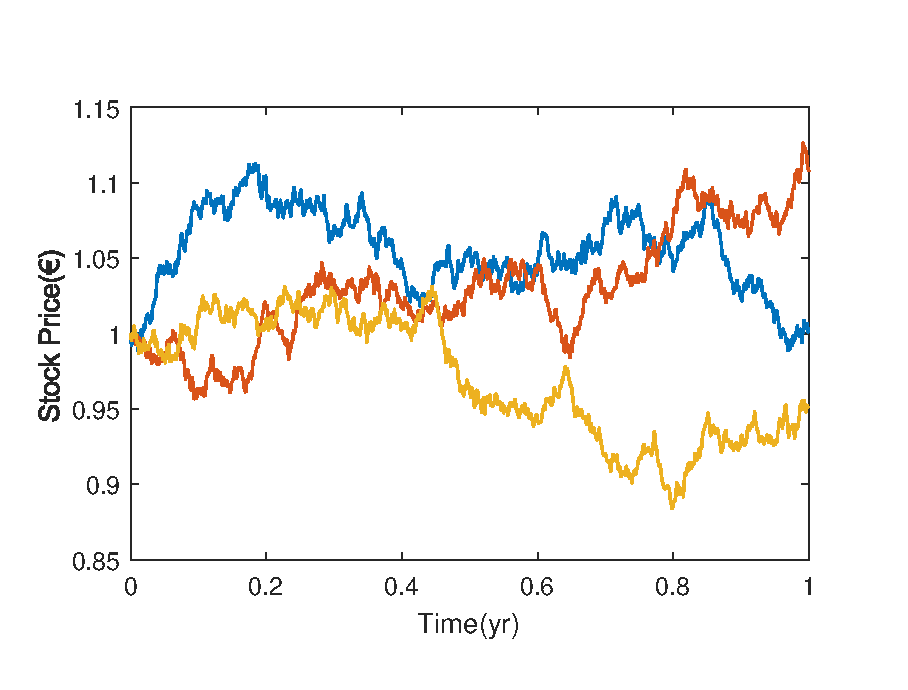
\includegraphics[width=0.9\columnwidth]{GBM.eps}
      \caption{Example of three GBM processes, using the parameters $r=\SI{0.06}{\per\year}$, $\sigma=0.05$, $S(0)=\SI{1}[\EUR]{}$ and time steps $\Delta t=10^{-3}\SI{}{\year}$.}\label{fig:GBM}
    \end{figure}




    
By simulating a large number of paths, some underlying tendencies might become apparent, which will prove useful in option pricing.


 American options, however, pose a much greater challenge.  Unlike European options, no analytic pricing model currently exists for this type of derivatives. Several numerical models have been proposed in the past in an attempt to solve this problem~\cite{Wilmott1,Hull}, such as the Longstaff-Schwartz algorithm~\citep{Longstaff}, which we shall approach in later sections of the present thesis.
\fi 
 
\section{Model Calibration}
\label{section:Model Calibration}
To calibrate SABR, we can either follow the Monte-Carlo approach and simulate a large number of paths, assuming stochastic volatility with some starting parameters and minimizing the difference between model-generated prices and real-world option prices, or we can use eq. xxx to obtain the implied volatility and minimize the market implied volatility.
